%%%%%%%%%%%%%%%%%%%%%%%%%%%%%%%%%%%%%%%%%%%%%%%%%%%%%%%%%%%%%%%%%%%%%%%%%%%%%%%%%%%%
% Document data
%%%%%%%%%%%%%%%%%%%%%%%%%%%%%%%%%%%%%%%%%%%%%%%%%%%%%%%%%%%%%%%%%%%%%%%%%%%%%%%%%%%%
\documentclass[12pt]{report} %report allows for chapters
\renewcommand\thesection{\arabic{section}} % ignore the title number for sections
%%%%%%%%%%%%%%%%%%%%%%%%%%%%%%%%%%%%%%%%%%%%%%%%%%%%%%%%%%%%%%%%%%%%%%%%%%%%%%%%%%%%




%%%%%%%%%%%%%%%%%%%%%%%%%%%%%%%%%%%%%%%%%%%%%%%%%%%%%%%%%%%%%%%%%%%%%%%%%%%%%%%%%%%%
% Packages
%%%%%%%%%%%%%%%%%%%%%%%%%%%%%%%%%%%%%%%%%%%%%%%%%%%%%%%%%%%%%%%%%%%%%%%%%%%%%%%%%%%%
\usepackage{color, soul, xcolor} % Colored text and highlighting, respectively

%Tikz
\usepackage{tikz-cd} % For commutative diagrams
\usepackage{tikz-3dplot}
\RequirePackage{pgfplots}
\usetikzlibrary{shadows}
\usetikzlibrary{shapes}
\usetikzlibrary{decorations}
\usetikzlibrary{arrows,decorations.markings} 
\usetikzlibrary{quotes,angles}

\usepackage{mathtools}
\usepackage{answers}
\usepackage{setspace}
\usepackage{graphicx}
\usepackage{enumerate}
\usepackage{multicol}
\usepackage{mathrsfs}
\usepackage[margin=1in]{geometry} 
\usepackage{amsmath,amsthm,amssymb}
\usepackage{marvosym,wasysym} %fucking smileys
\usepackage{subcaption}
\usepackage{morefloats}
\usepackage{float}
\usepackage{hyperref}
\usepackage{listings} %inputting code
\lstloadlanguages{[5.2]Mathematica} %same
%%%%%%%%%%%%%%%%%%%%%%%%%%%%%%%%%%%%%%%%%%%%%%%%%%%%%%%%%%%%%%%%%%%%%%%%%%%%%%%%%%%%




%%%%%%%%%%%%%%%%%%%%%%%%%%%%%%%%%%%%%%%%%%%%%%%%%%%%%%%%%%%%%%%%%%%%%%%%%%%%%%%%%%%%
% Shortcuts
%%%%%%%%%%%%%%%%%%%%%%%%%%%%%%%%%%%%%%%%%%%%%%%%%%%%%%%%%%%%%%%%%%%%%%%%%%%%%%%%%%%%
% Number systems
\newcommand{\N}{\mathbb{N}}
\newcommand{\Z}{\mathbb{Z}}
\newcommand{\C}{\mathbb{C}}
\newcommand{\R}{\mathbb{R}}
\newcommand{\Q}{\mathbb{Q}}
\newcommand{\partialx}{\frac{\partial f}{\partial x}}
\newcommand{\partialy}{\frac{\partial f}{\partial y}}
\newcommand{\partialz}{\frac{\partial f}{\partial z}}

% Operators/functions
\newcommand{\id}{\mathrm{Id}}
\newcommand{\RE}{\mathrm{Re}}
\newcommand{\IM}{\mathrm{Im}}
\DeclareMathOperator{\sech}{sech}
\DeclareMathOperator{\csch}{csch}
%%%%%%%%%%%%%%%%%%%%%%%%%%%%%%%%%%%%%%%%%%%%%%%%%%%%%%%%%%%%%%%%%%%%%%%%%%%%%%%%%%%%




%%%%%%%%%%%%%%%%%%%%%%%%%%%%%%%%%%%%%%%%%%%%%%%%%%%%%%%%%%%%%%%%%%%%%%%%%%%%%%%%%%%%
% Environments
%%%%%%%%%%%%%%%%%%%%%%%%%%%%%%%%%%%%%%%%%%%%%%%%%%%%%%%%%%%%%%%%%%%%%%%%%%%%%%%%%%%%
% Italic font
\newtheorem{theorem}{Theorem}[section]
\newtheorem{lemma}{Lemma}[section]
\newtheorem{corollary}{Corollary}[section]
\newtheorem{axiom}{Axiom}

% Plain font
\theoremstyle{definition}
\newtheorem{definition}{Definition}[section]
\newtheorem{example}{Example}[section]
\newtheorem{remark}{Remark}[section]
\newtheorem{solution}{Solution}
\newtheorem{problem}{Problem}[section]
\newtheorem{question}{Question}[section]
\newtheorem{answer}{Answer}[section]
\newtheorem{exercise}{Exercise}[section]
%%%%%%%%%%%%%%%%%%%%%%%%%%%%%%%%%%%%%%%%%%%%%%%%%%%%%%%%%%%%%%%%%%%%%%%%%%%%%%%%%%%%

\begin{document}


\begin{center}
   \textsc{\large MATH 255, Homework 5: \emph{Solutions}}\\
\end{center}
\vspace{.5cm}

\noindent\textbf{Relevant Sections:} 8.4, 8.7, 9.1, 9.2, 9.8, 16.7, 10.3 \\

\noindent\textbf{Problem 1.} Integrate the following.
\begin{enumerate}[(a)]
    \item $f(z)=\frac{1}{z}$ about the contour $\gamma(t)=e^{2\pi it}$ from $t=0$ to $t=1$.
    \item $g(z)=z^2$ about the contour $\gamma(t)=t+it$ from $t=0$ to $t=5$.
\end{enumerate}

\begin{solution}~
Recall we have that
\[
\int_\gamma f(\gamma) d\gamma = \int_{t_0}^{t_1} f(\gamma(t))\gamma'(t)dt.
\]
\begin{enumerate}[(a)]
    \item Here we have $\gamma'(t)=2\pi i e^{2\pi i t}$ and $f(\gamma(t))=\frac{1}{e^{2\pi i t}}$. We plug these in and get
    \[
    \int_0^1 \frac{1}{e^{2\pi i t}} \cdot 2\pi i e^{2\pi i t}dt.
    \]
    This simplifies quite a bit, and we can work this out fairly easily
    \begin{align*}
        \int_0^1 \frac{1}{e^{2\pi i t}} \cdot 2\pi i e^{2\pi i t}dt & = 2\pi i \int_0^1 \frac{e^{2\pi i t}}{e^{2\pi i t}} dt \\
        &= 2\pi i \int_0^1 dt\\
        &= \left. 2 \pi i t \right|_0^1 = 2\pi i.
    \end{align*}
    Without going into details, this result is very important in the study of complex functions.  If you're interested, try, instead, $f(z)=\frac{1}{z^n}$.
    \item Here we have $\gamma'(t)=1+i$ and 
    \[
    f(\gamma(t))=(t+it)^2 = t^2+2it^2-t^2 = 2it^2.
    \]
    So we integrate
    \begin{align*}
        \int_0^5 (2it^2)(1+i)dt&= 2i(1+i)\int_0^5 t^2 dt\\
        &= \left. (-2+2i) \frac{t^3}{3}\right|_0^5\\
        &= \frac{5^3}{3}(-2+2i)\\
        &= -\frac{-250}{3}+\frac{250i}{3}.
    \end{align*}
\end{enumerate}
\end{solution}

\noindent\textbf{Problem 2.} Plot the following curves and print pictures of each using the following: \url{https://christopherchudzicki.github.io/MathBox-Demos/parametric_curves_3D.html}. The blue curve will be the path the particle follows over the given time range and the black arrow will be the vector pointing to the position of the particle in space at a given time $t$.
\begin{enumerate}[(a)]
    \item (Helix) $\gamma_1(t)=(3\cos(t),3\sin(t),t)$ from $t=0$ to $t=2\pi$. Where might this show up? If you think about the Earth moving through space and the Moon orbiting Earth, then the Moon follows a helical path.
    \item (Falling Ball) $\gamma_2(t)=(t,0.5t, 9-t^2)$ from $t=0$ to $t=3$.
    \item (Perturbed Orbiter) $\gamma_3(t)=(3\cos(t),3\sin(t),\sin(10t))$ from $t=0$ to $t=2\pi\approx 6.28$. 
\end{enumerate}
The point of this is to get a feel for different curves in space.  So plot another interesting curve of your choice and tell me what equations you used.

\begin{solution}~
\begin{enumerate}[(a)]
    \item Here is the plot.
    \begin{figure}[H]
        \centering
        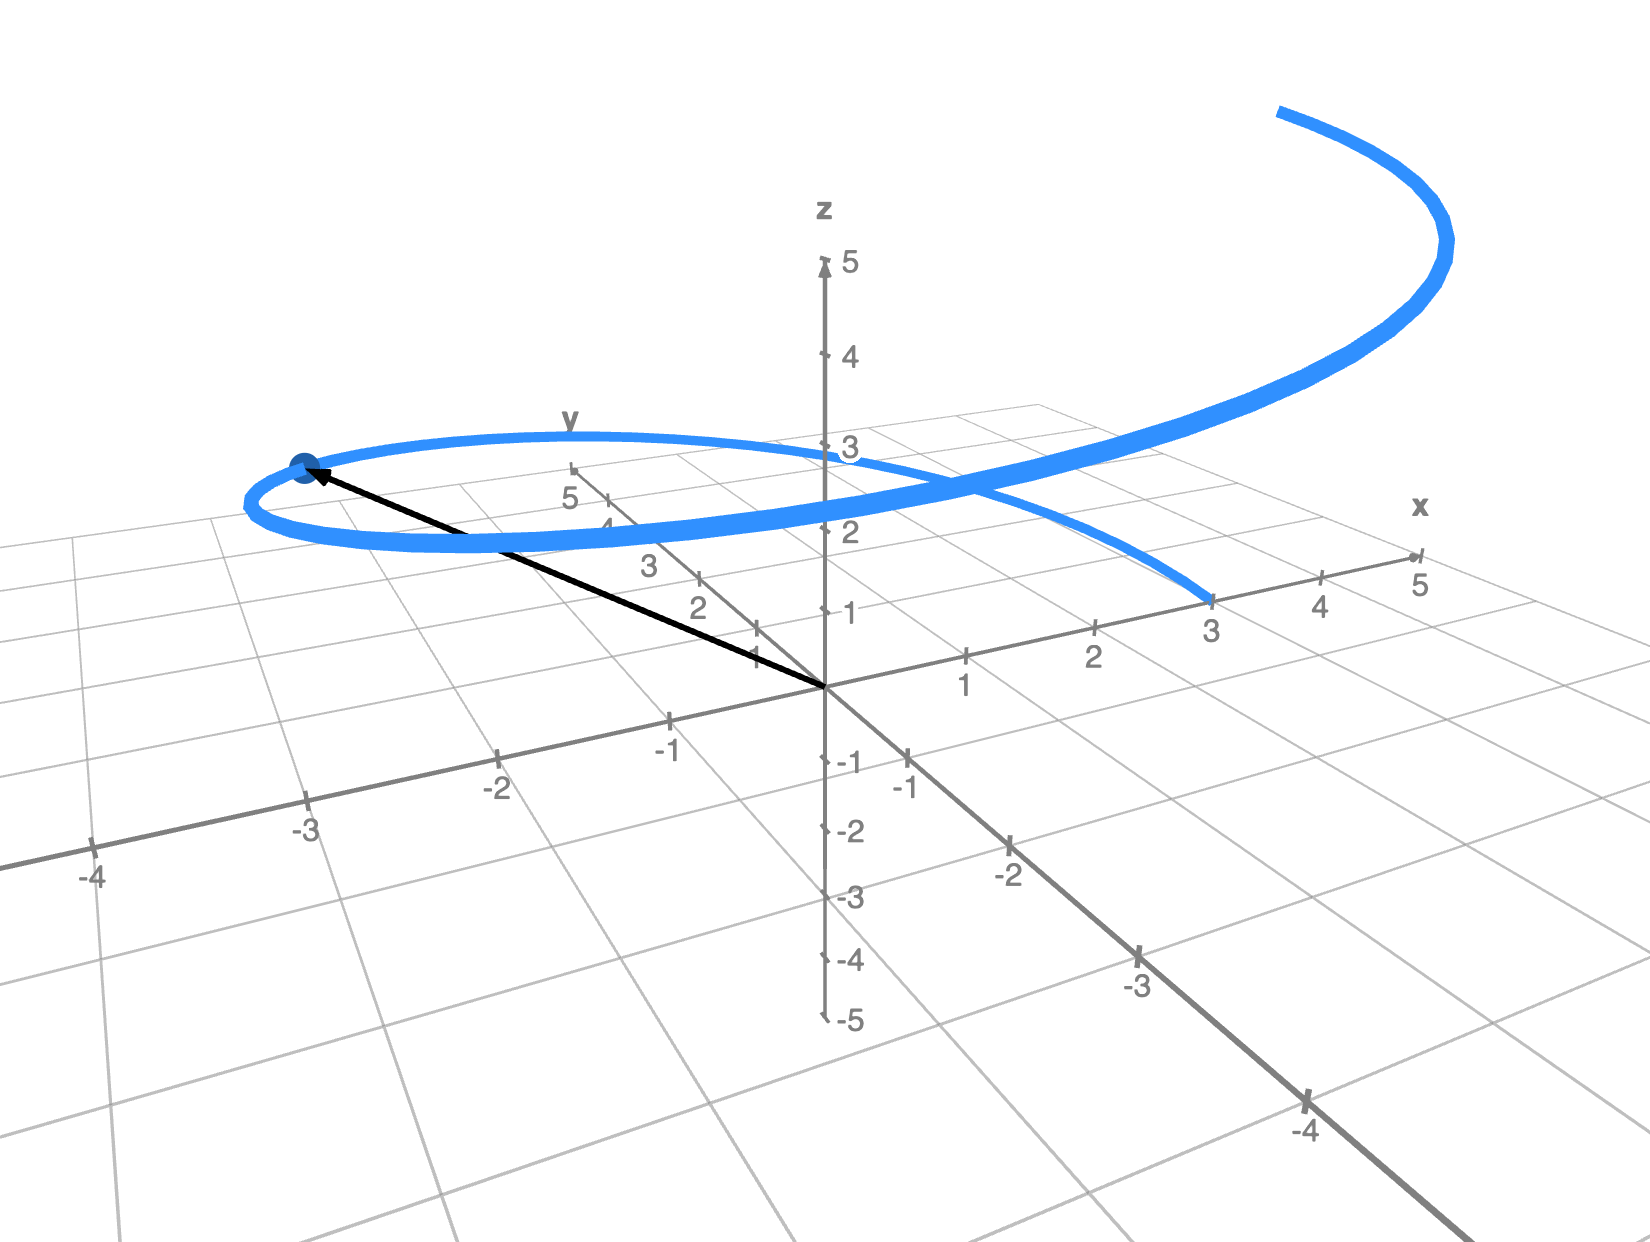
\includegraphics[width=.6\textwidth]{Images/helix.png}
        \caption{Helix.}
    \end{figure}
    \item Here is the plot.
    \begin{figure}[H]
        \centering
        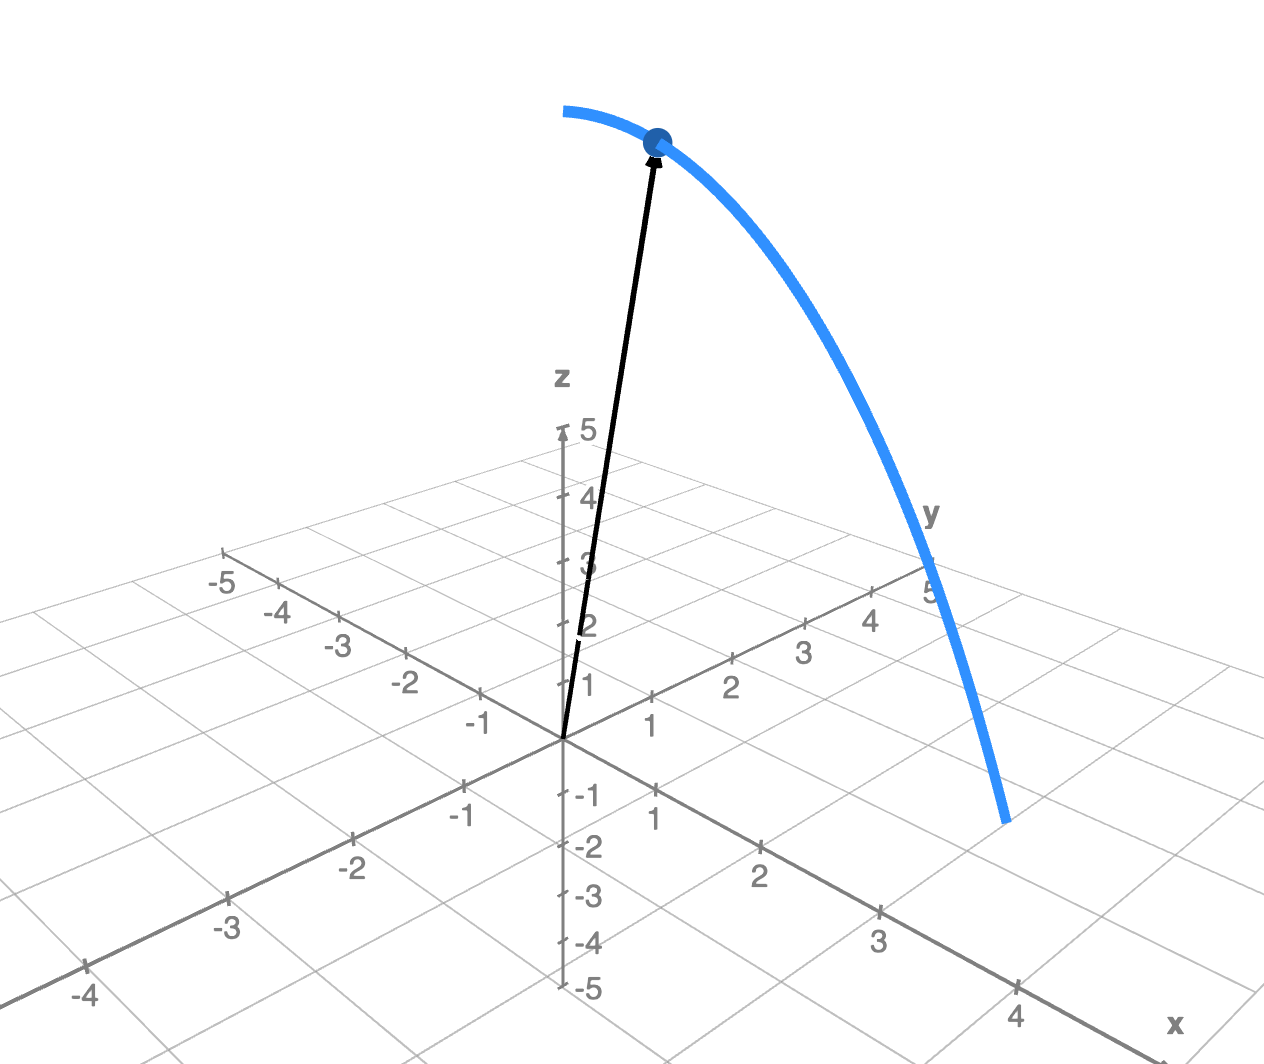
\includegraphics[width=.6\textwidth]{Images/falling_ball.png}
        \caption{Falling ball.}
    \end{figure}
    \item Here is the plot.
    \begin{figure}[H]
        \centering
        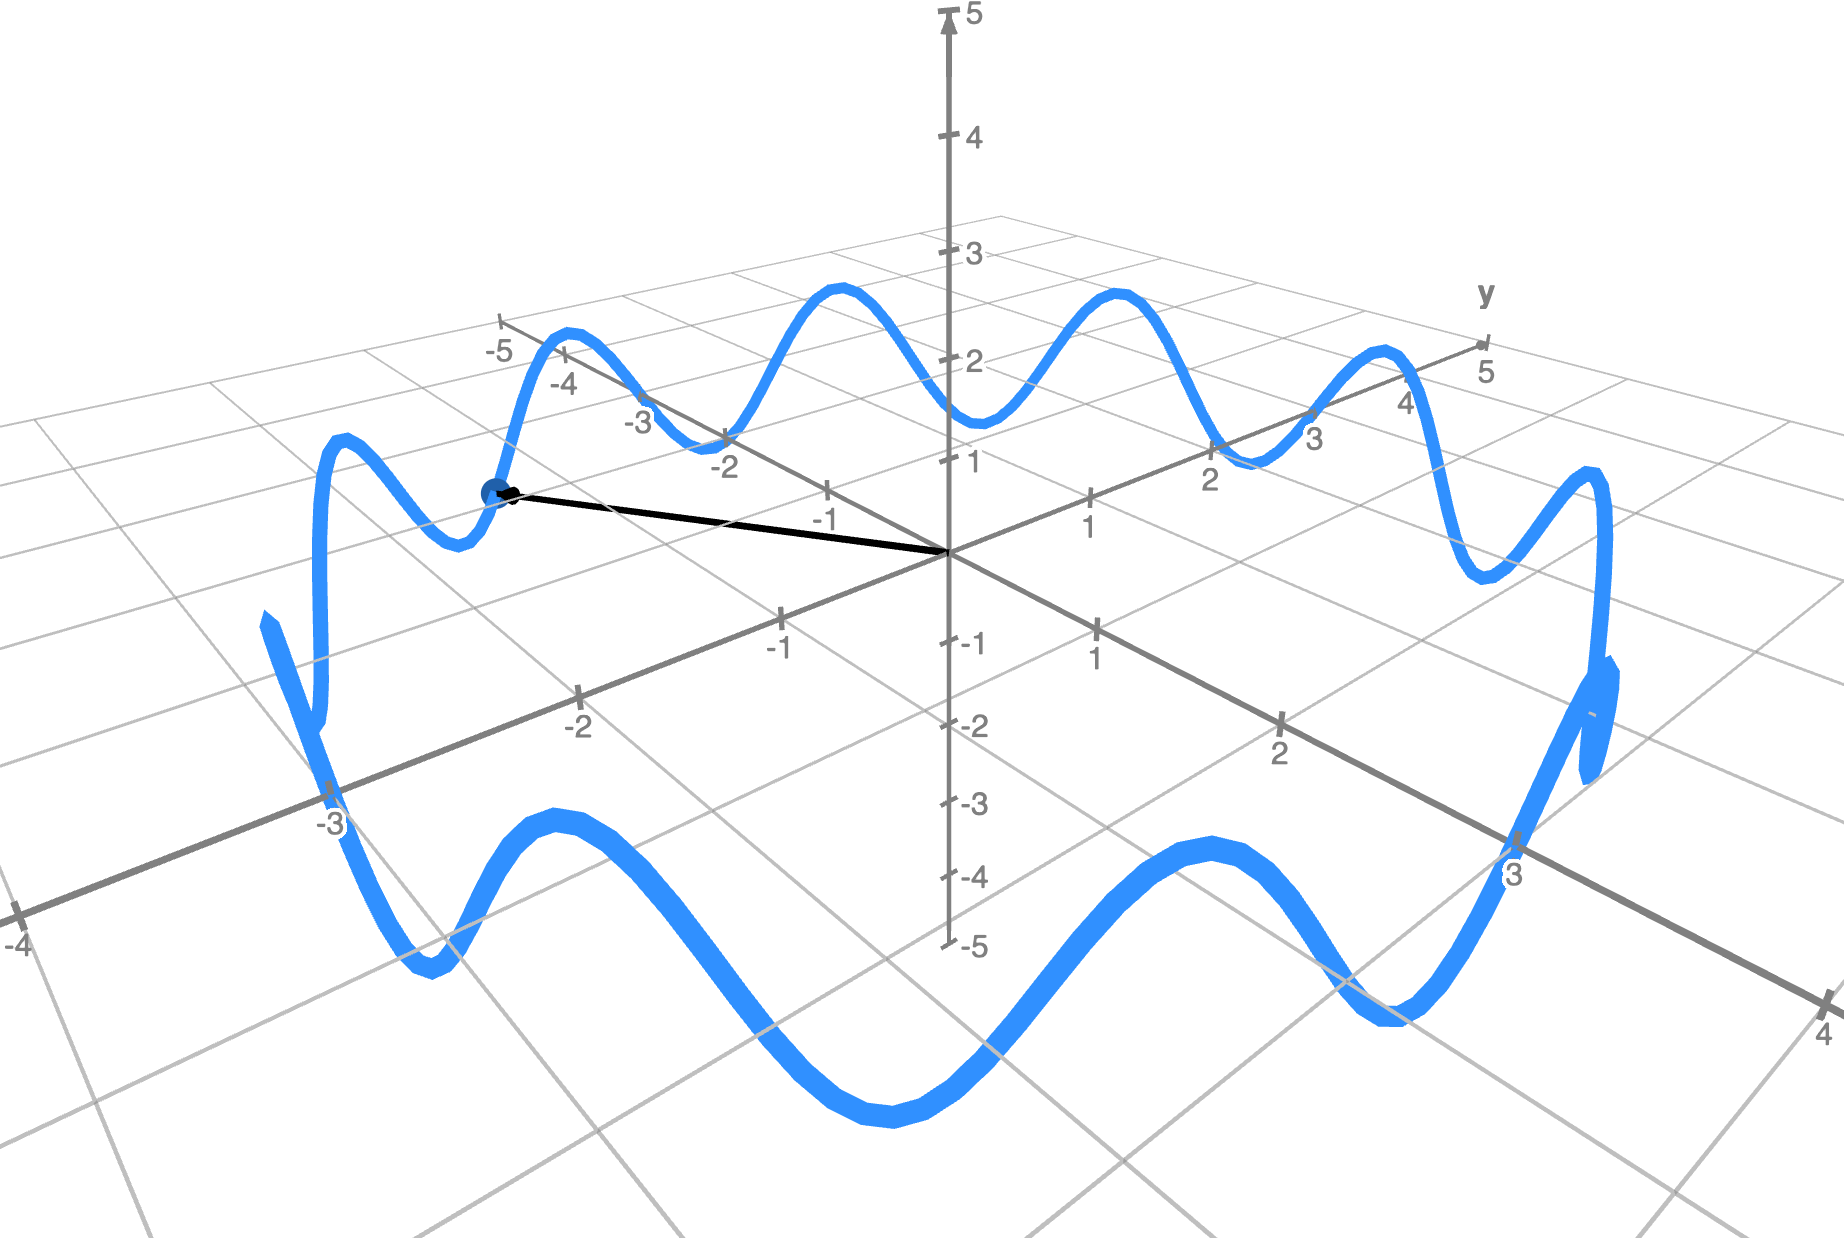
\includegraphics[width=.6\textwidth]{Images/perturbed_orbiter.png}
        \caption{Perturbed orbiter.}
    \end{figure}
\end{enumerate}
And an extra plot of my own.
\begin{figure}[H]
    \centering
    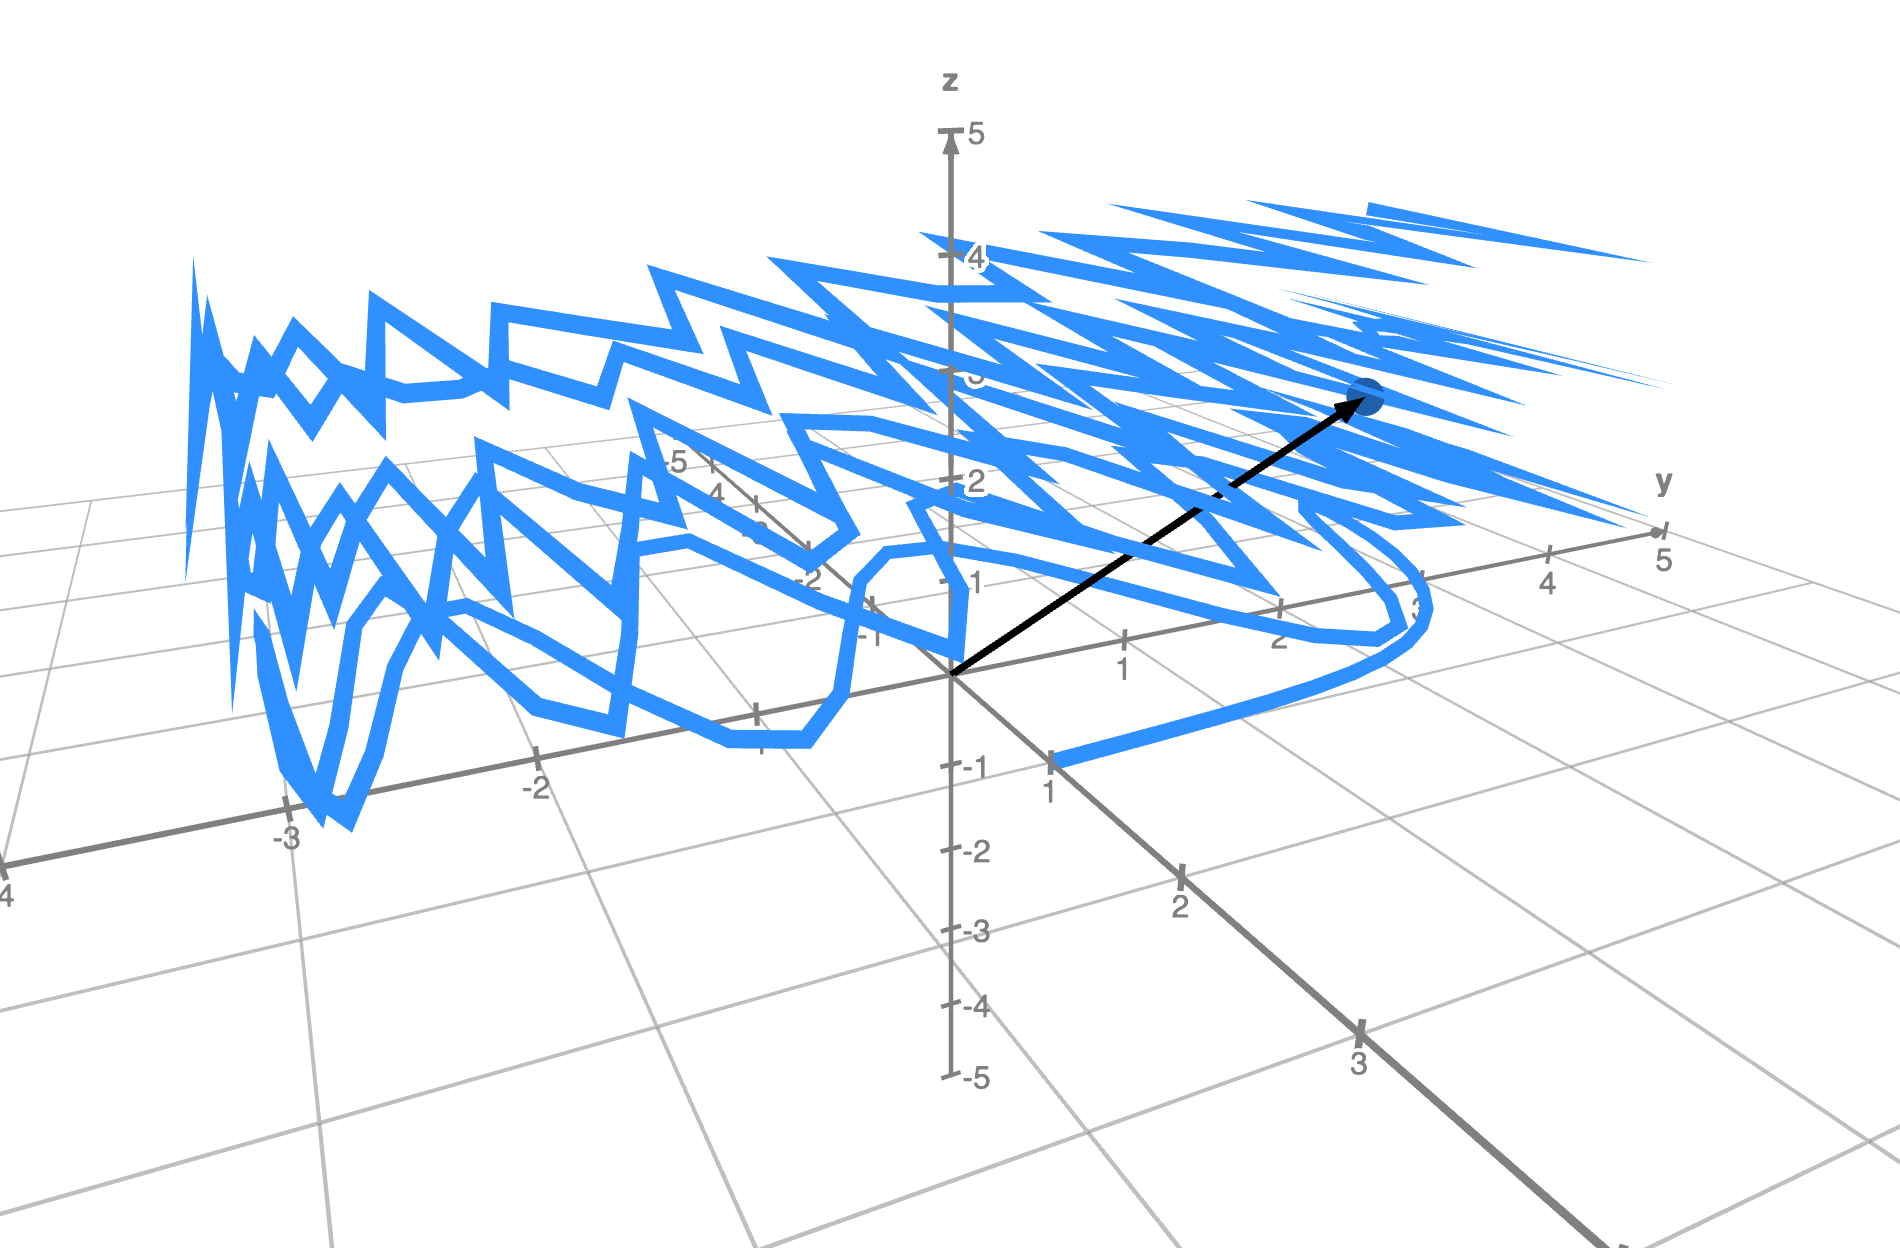
\includegraphics[width=.6\textwidth]{Images/random_curve.png}
    \caption{Something kind of random.}
\end{figure}
\end{solution}

\noindent\textbf{Problem 3.} The length of a curve is an important notion.  In fact, the length of a curve is often very much related to the energy of some configuration.  We can compute the length of a curve over the time $t=t_0$ to $t=t_1$ by integrating the \emph{speed} of the curve over that time. 
\[
l(\gamma)= \int_{t_0}^{t_1} \|\gamma'(t)\|dt.
\]
We can find the \emph{energy} of this curve by taking
\[
E(\gamma)= \int_{t_0}^{t_1} \frac{1}{2}\|\gamma'(t)\|^2dt.
\]
\begin{enumerate}[(a)]
    \item Find the length of the Helix from Problem 2 (a). 
    \item Using WolframAlpha (when necessary) find the energy of the Perturbed Orbiter in Problem 2 (c). Roughly, this corresponds to the potential energy a rubber band stretched this way would have. 
\end{enumerate}

\begin{solution}~
\begin{enumerate}[(a)]
    \item We let $\gamma(t) = (3\cos (t), 3\sin(t), t)$ and we go from $t=0$ to $t=2\pi$. Then we have
\[
\gamma'(t) = (-3\sin(t),3\cos(t),1)
\]
and so
\[
\|\gamma'(t)\| = \sqrt{(-3\sin (t))^2+(3\cos (t))^2+1^2} = \sqrt{10},
\]
since $\sin^2(t)+\cos^2(t)=1$ (this is an identity you need to remember).

Now we integrate to find
\begin{align*}
    l(\gamma) &= \int_0^{2\pi} \sqrt{10}dt\\
    &= \sqrt{10} t|_0^{2\pi}\\
    &= 2\pi \sqrt{10}.
\end{align*}
    \item Here we have $\gamma(t)=(3\cos(t),3\sin(t),\sin(10t))$ starting from $t=0$ to $t=2\pi$. Then we have
    \[
    \gamma'(t)=(-3\sin(t),3\cos(t),10\cos(10t))
    \]
    and so
    \[
    \|\gamma'(t)\| = \sqrt{(-3\sin(t))^2+(3\cos(t))^2+(10\cos(10t))^2} = \sqrt{9+100\cos^2(10t)}.
    \]
    This is not a function that can be integrated without some trigonometric substitutions.  If you're interested, you can look at integration using trigonometric substitutions, but I will not go into it.  
    Instead, I'd argue it's good practice for us to get more used to using technology to help solve our problems.  So, we wish to evaluate the integral
    \[
    E(\gamma) = \int_0^{2\pi} \frac{1}{2}(9+100\cos^2(10t))dt.
    \]
    What I did was went to WolframAlpha and typed in
    \begin{center}
    \begin{lstlisting}
Integrate[(1/2)*(9+100cos^2(10t)),{t,0,2pi}]
\end{lstlisting}
    \end{center}
    What this syntax says is to integrate our function 
    \[
    \frac{1}{2}(9+100\cos^2(10t))
    \]
    with respect to $t$ from $0$ to $2\pi$ (that is the $\{t,0,2\pi\}$ portion).
    
    Using this, we find
    \[
    E(\gamma)=59\pi.
    \]

\end{enumerate}
\end{solution}

\noindent\textbf{Problem 4.} Given a function $F(x,y)$, we can create an object called the \emph{graph} of $F(x,y)$ by plotting $(x,y,F(x,y))$.  In fact, you have done this many times in your life.  For example, you have consistently plotted the graph of a function $f(x)$ by plotting $(x,f(x))$ in the plane.  

For the following functions, use \url{https://www.monroecc.edu/faculty/paulseeburger/calcnsf/CalcPlot3D/} to plot the graphs.  Print them off and include them and describe what the graph of the function does as we move along the $x$-axis, $y$-axis, and along the line $y=x$. For each graph, use the range $-3\leq x \leq 3$ and $-3\leq y \leq 3$.
\begin{enumerate}[(a)]
    \item $F(x,y)=\frac{4xy}{1+x^2+y^2}$.
    \item $G(x,y)=\sin(xy)$.
    \item $H(x,y)=\frac{-x^2-y^2}{5}$.
\end{enumerate}
If you'd like, you can think of these functions as the height of a sheet above the $xy$-plane.  Or you could consider these to be a temperature distribution (the temperature at each point $(x,y)$) on the plane as well.

\begin{solution}~
\begin{enumerate}[(a)]
    \item 
    \begin{figure}[H]
        \centering
        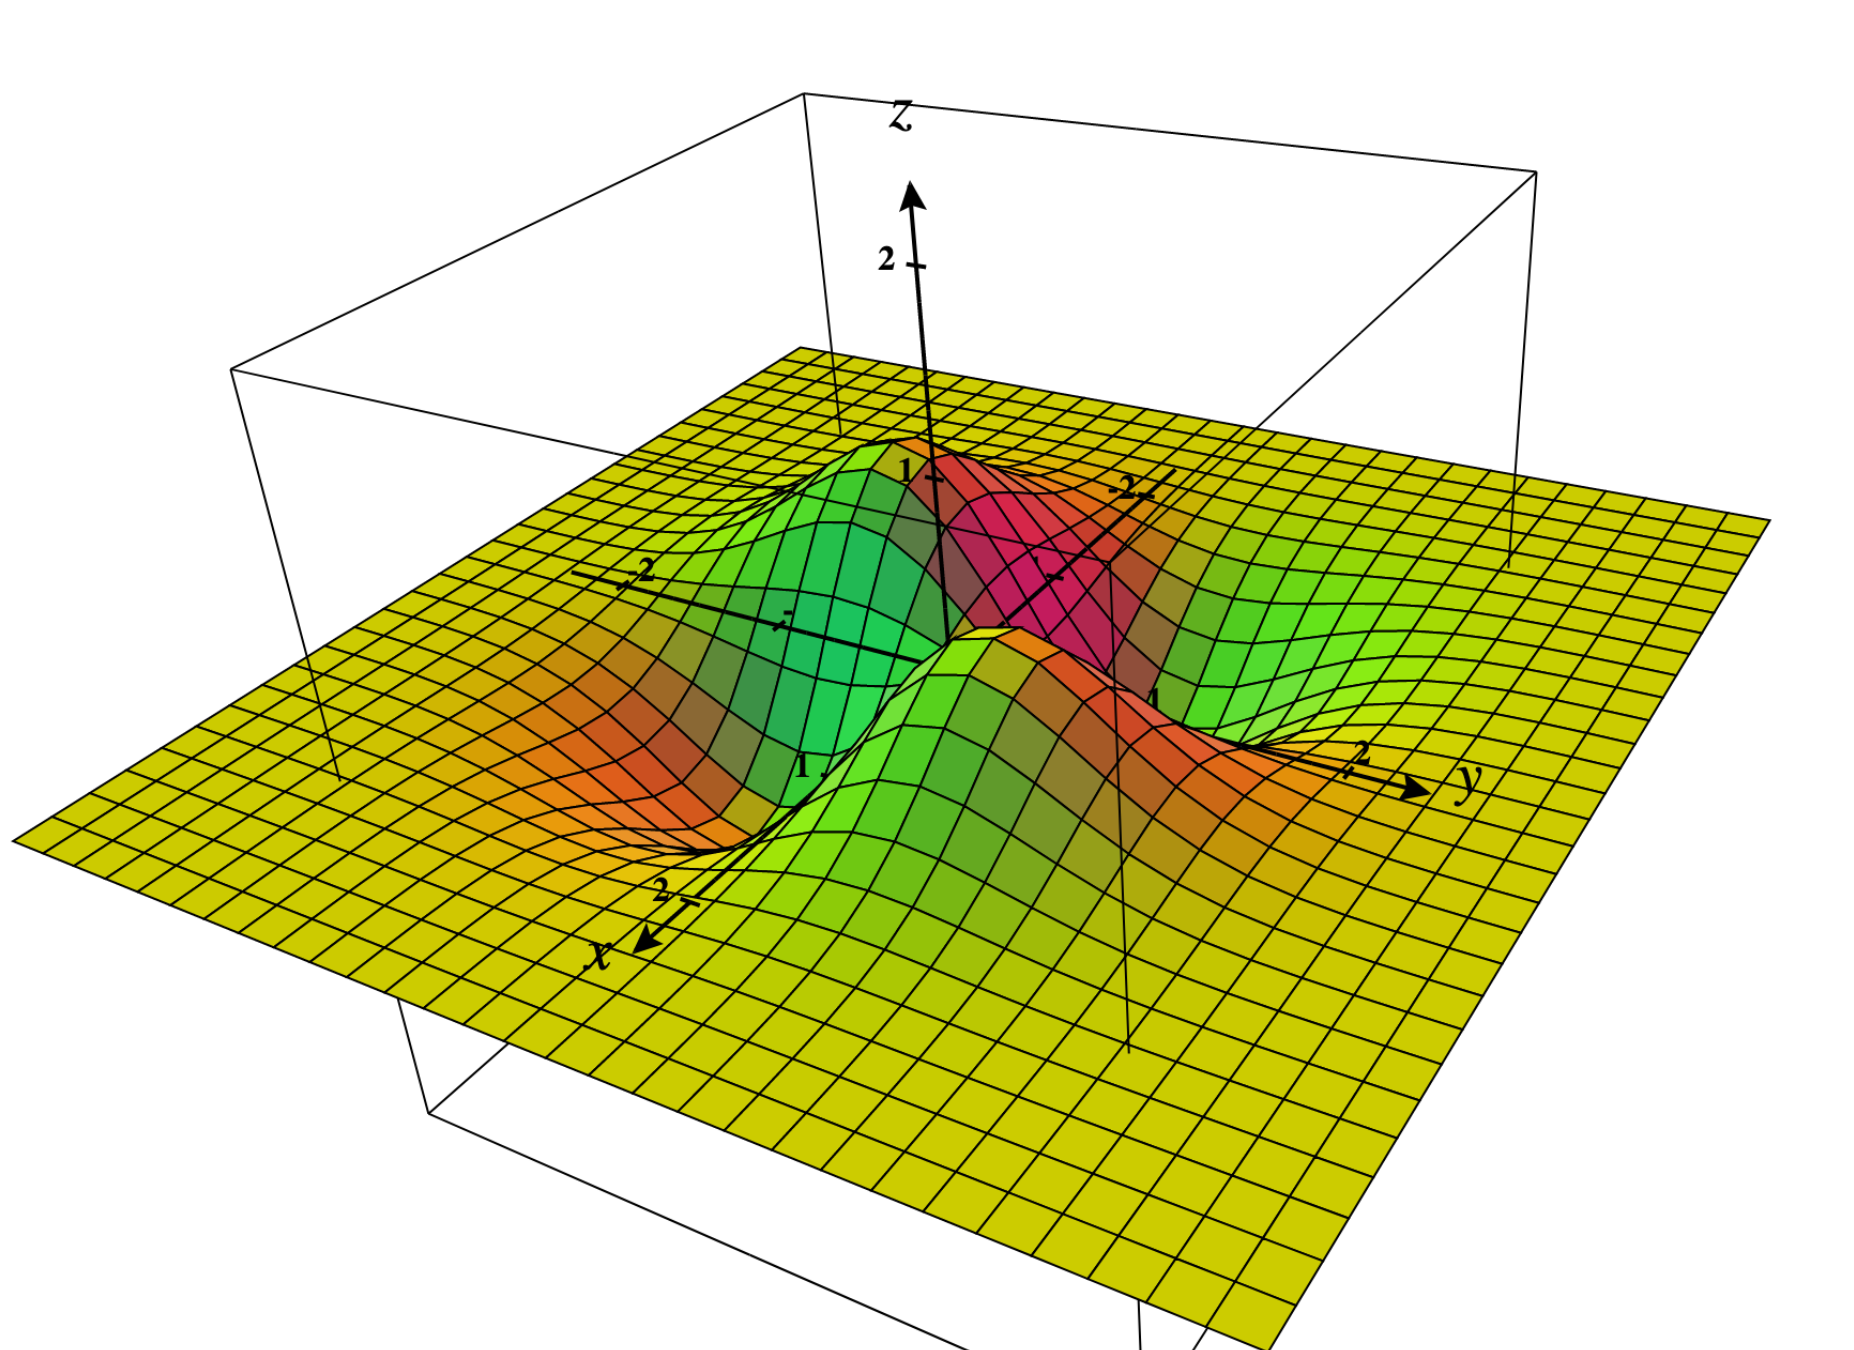
\includegraphics[width=.6\textwidth]{Images/4a.png}
        \caption{The graph of $F(x,y)$.}
    \end{figure}
    \item
    \begin{figure}[H]
        \centering
        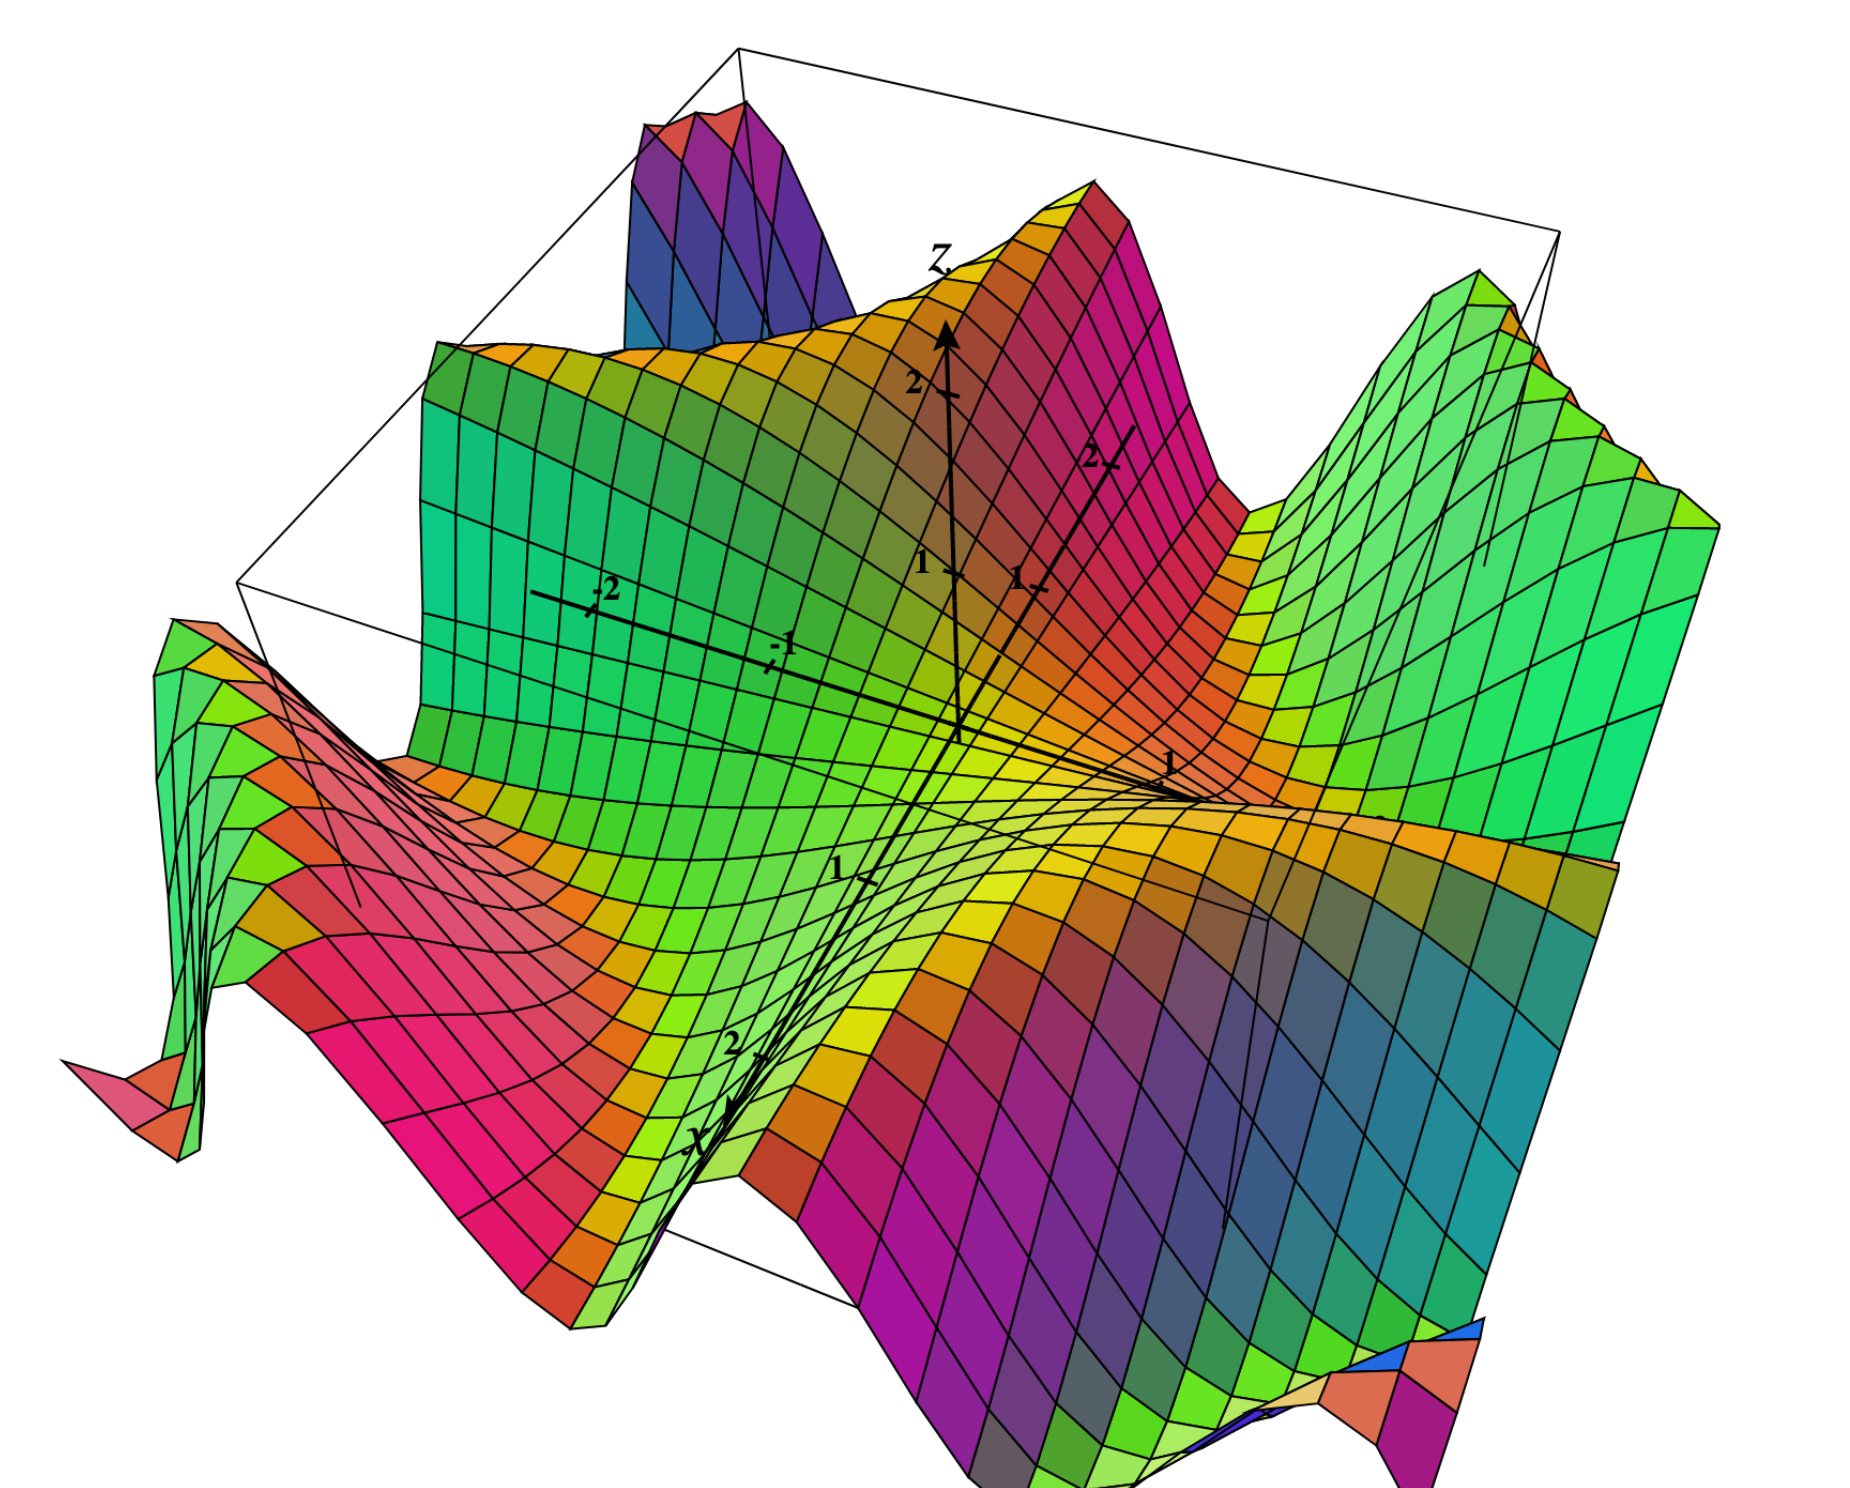
\includegraphics[width=.6\textwidth]{Images/4b.png}
        \caption{The graph of $G(x,y)$.}
    \end{figure}
    \item
    \begin{figure}[H]
        \centering
        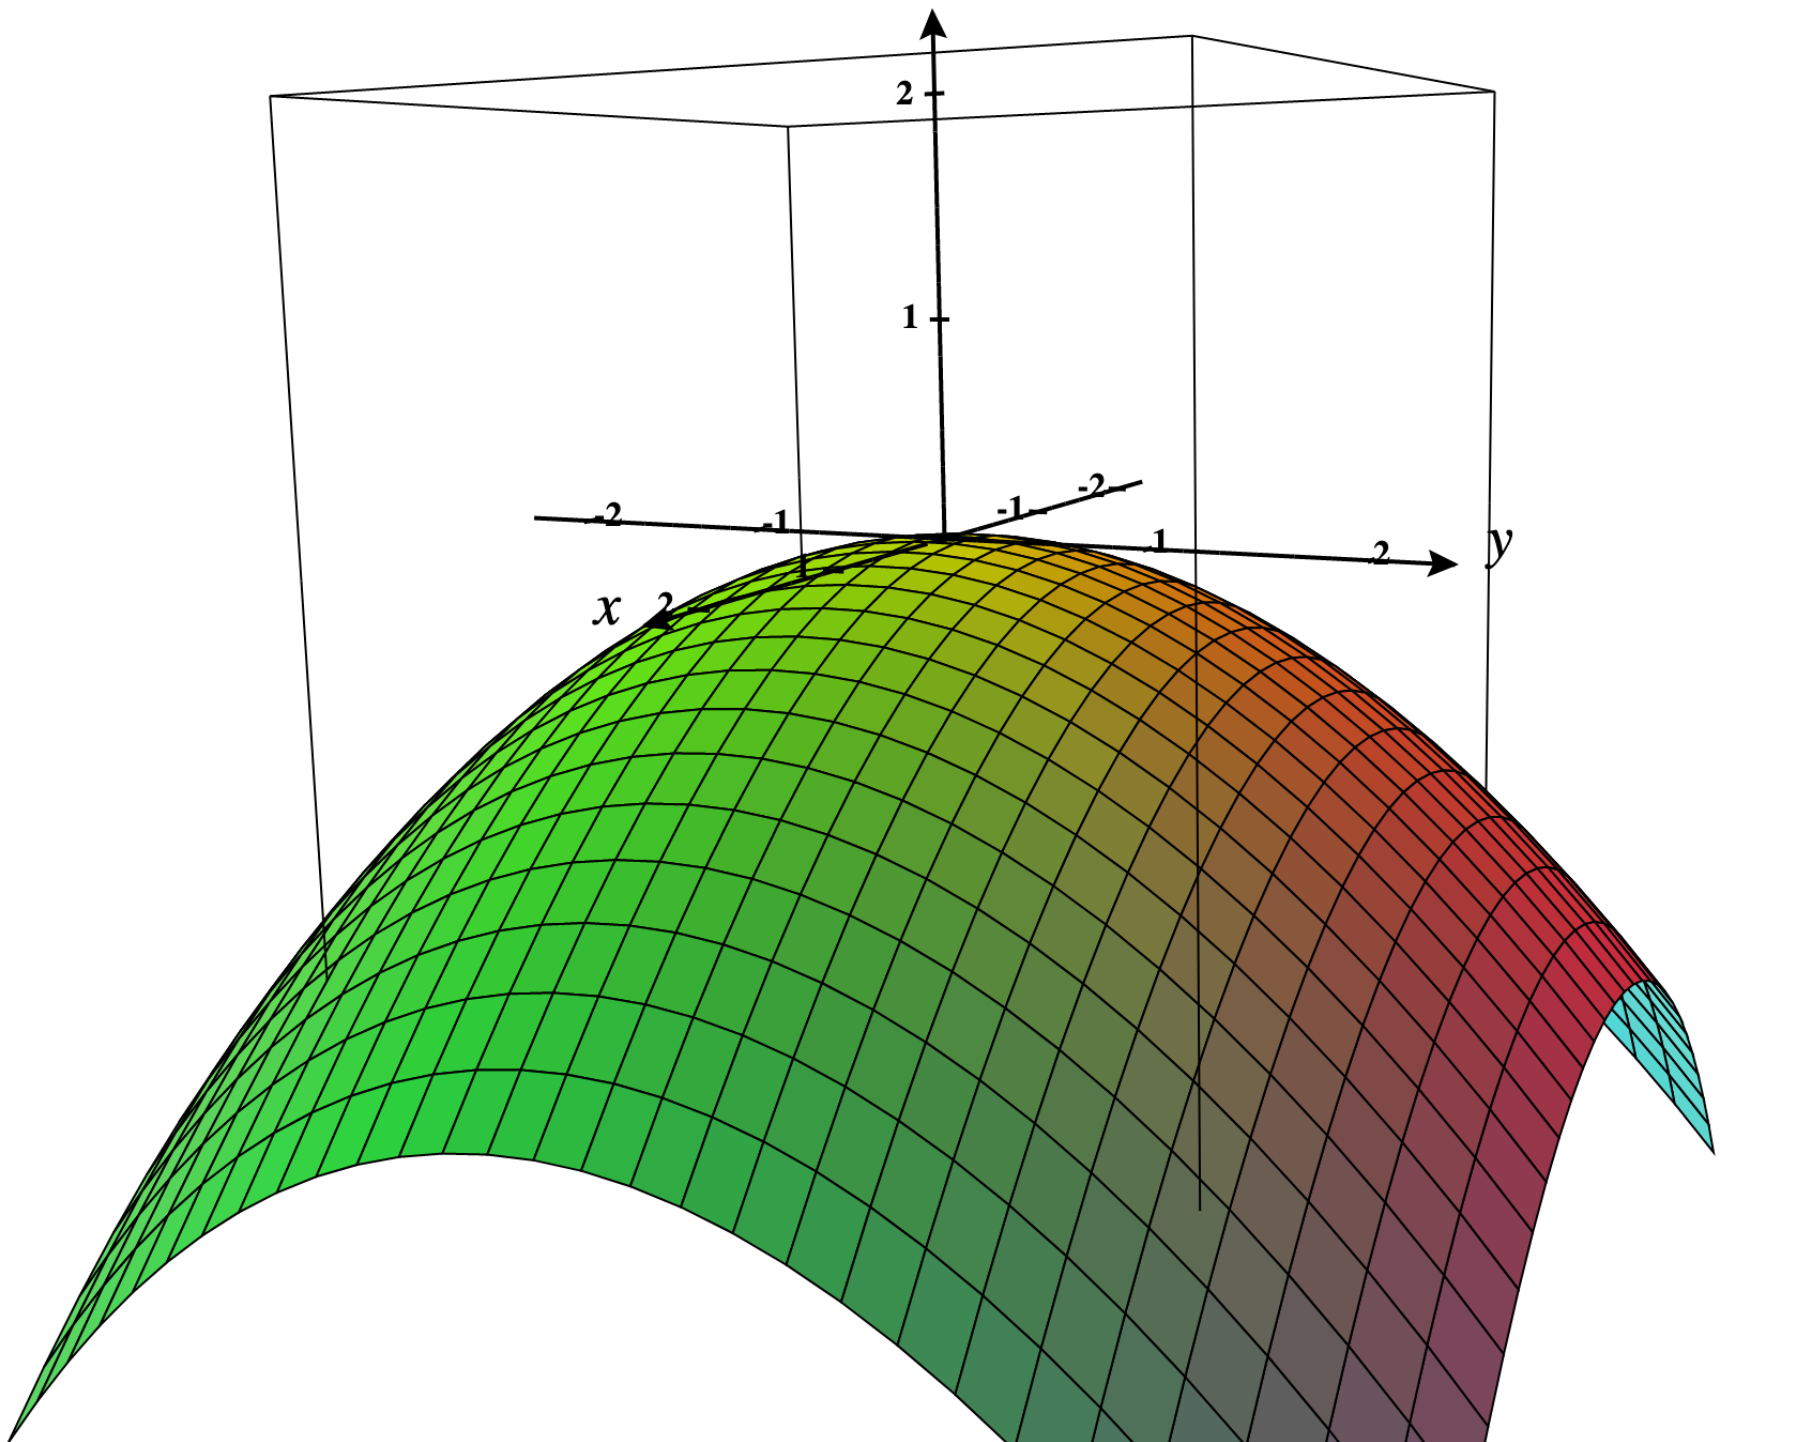
\includegraphics[width=.6\textwidth]{Images/4c.png}
        \caption{The graph of $H(x,y)$.}
    \end{figure}
\end{enumerate}
\end{solution}

\noindent\textbf{Problem 5.} Many times in life we wish to model equations that describe the directional (vector) flow of material as opposed to just a single scalar quantity like temperature.  For example, you could describe the wind speed and direction at each point in space outside or the velocity of water flow at each point inside of a pipe. 

To visualize this, visit \url{https://www.geogebra.org/m/u3xregNW}.  What this program will do is place an arrow at each point in 3D space with coordinates $(x,y,z)$.  The arrow is a vector at a point $(x,y,z)$ that we often denote by
\[
\mathbf{v}(x,y,z)
\]
and call a \emph{vector field}. If you pick a starting point $(x,y,z)$ you can follow the arrows along and this will give you the path that, for example, a small particle would follow in a windy day.

Plot the following vector fields and print them out.
\begin{enumerate}[(a)]
    \item (Constant wind from the northwest) $\mathbf{v}(x,y,z)=(1,-1,0)$.
    \item (Two wind fronts meeting) $\mathbf{w}(x,y,z)=(y,x,0)$.
    \item (Explosion) $\mathbf{u}(x,y,z)=(x,y,z)$.
    \item (Whirlpool) $\mathbf{r}(x,y,z)=\left(\frac{-y}{x^2+y^2},\frac{x}{x^2+y^2},0\right).$
\end{enumerate}
Notice that most of these have 0 $z$-component.  For those, feel free to use \url{https://www.desmos.com/calculator/eijhparfmd} to visualize these.  It may look a bit nicer.

\begin{solution}~
\begin{enumerate}[(a)]
    \item 
    \begin{figure}[H]
        \centering
        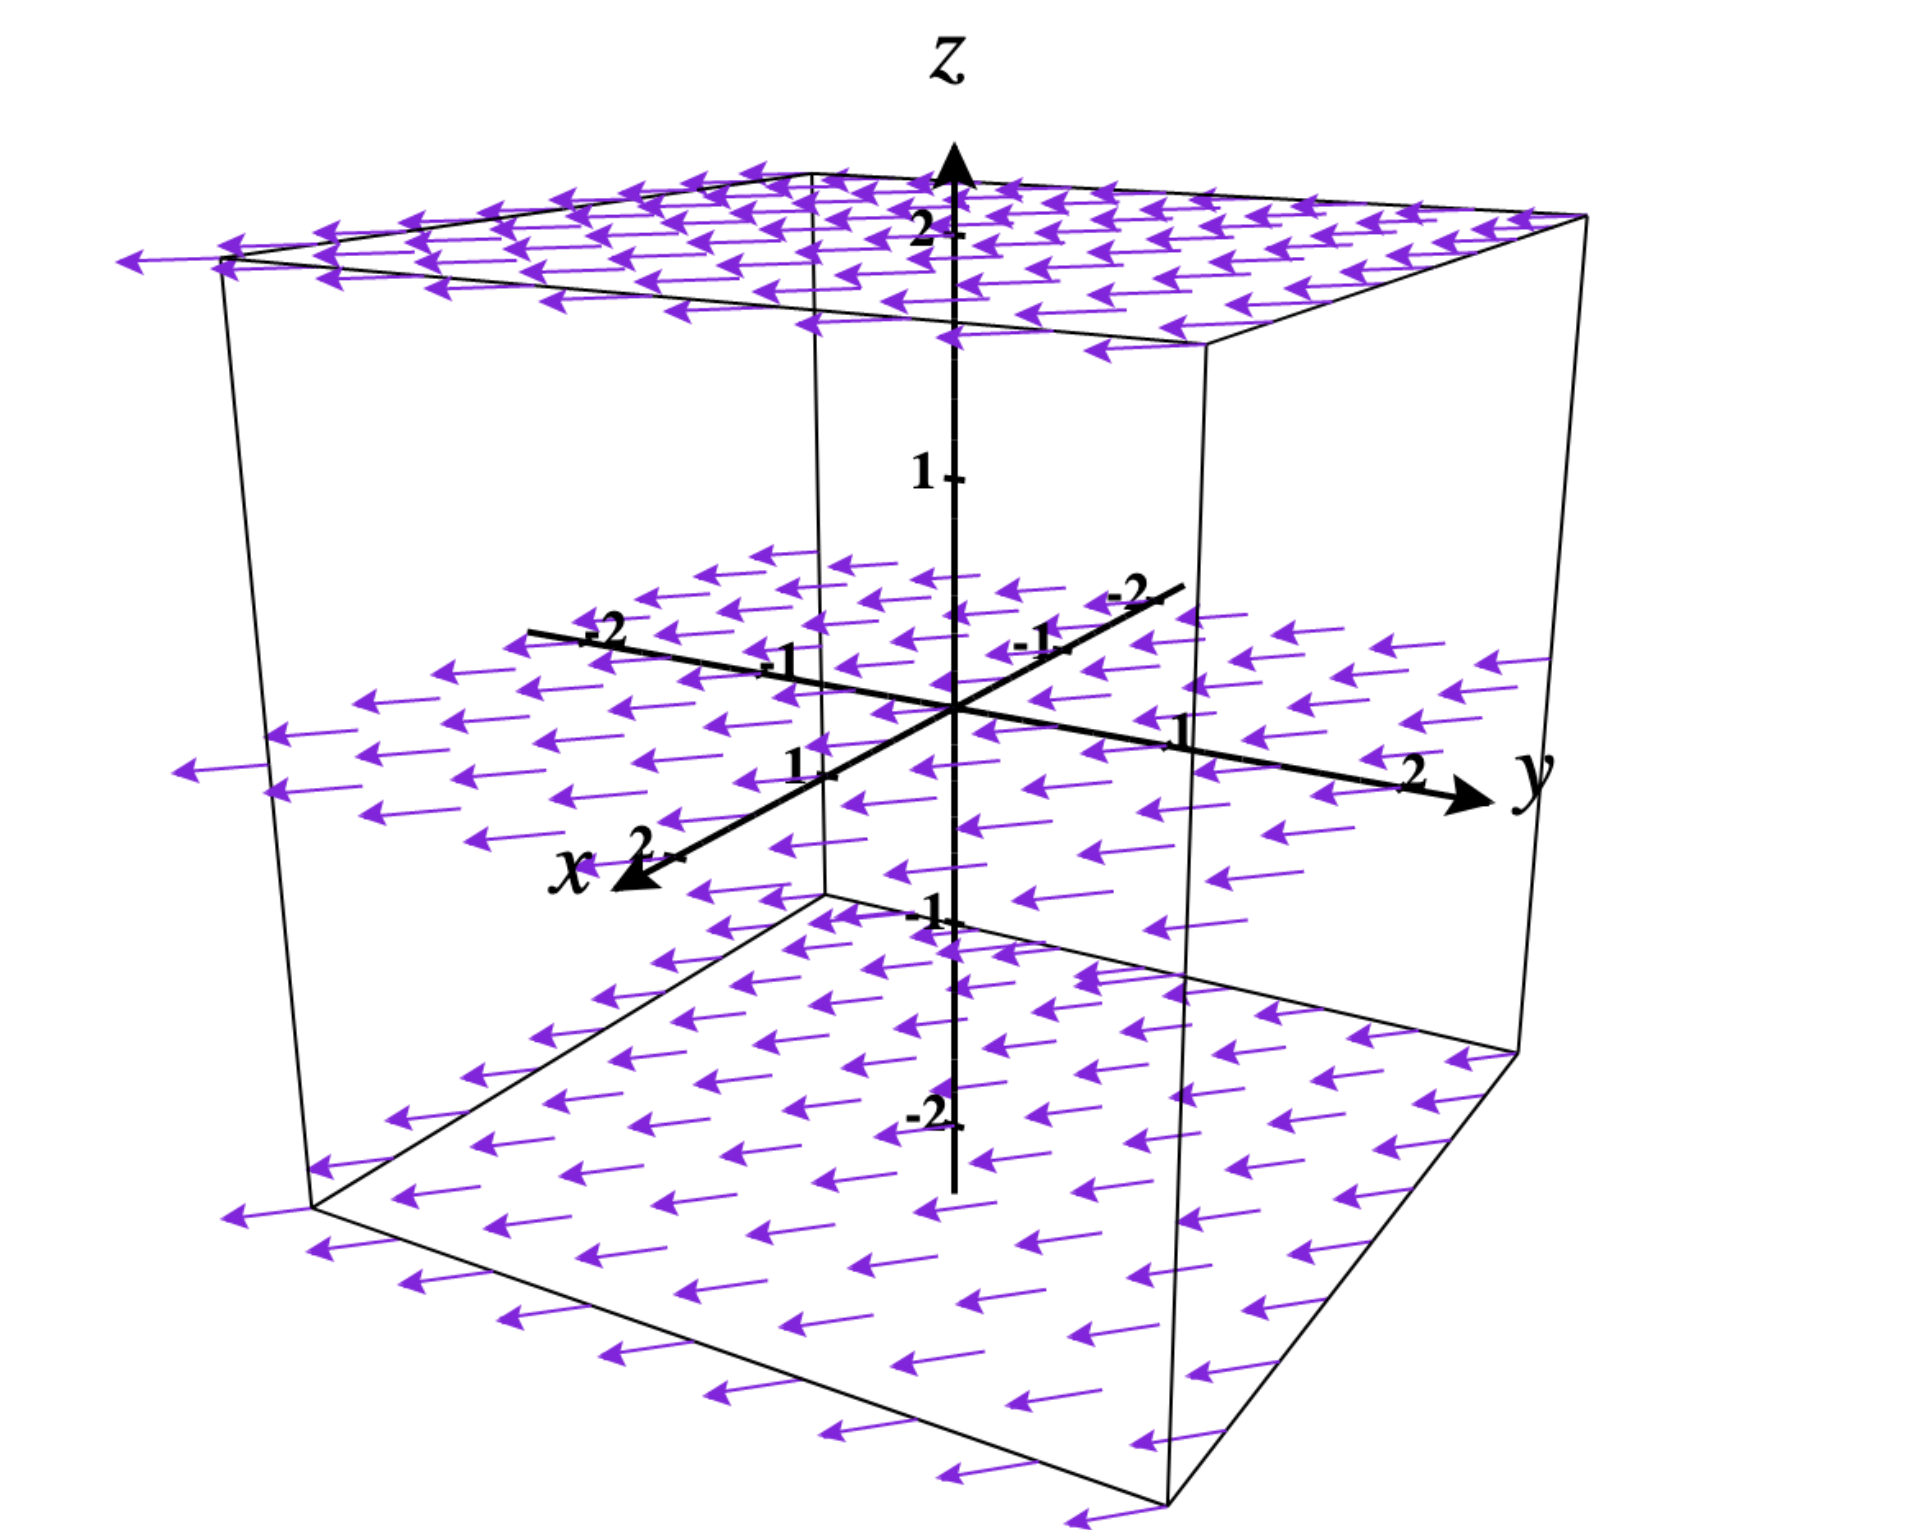
\includegraphics[width=.6\textwidth]{Images/5a.png}
        \caption{Plot for $\mathbf{v}(x,y,z)$.}
    \end{figure}
    \item 
    \begin{figure}[H]
        \centering
        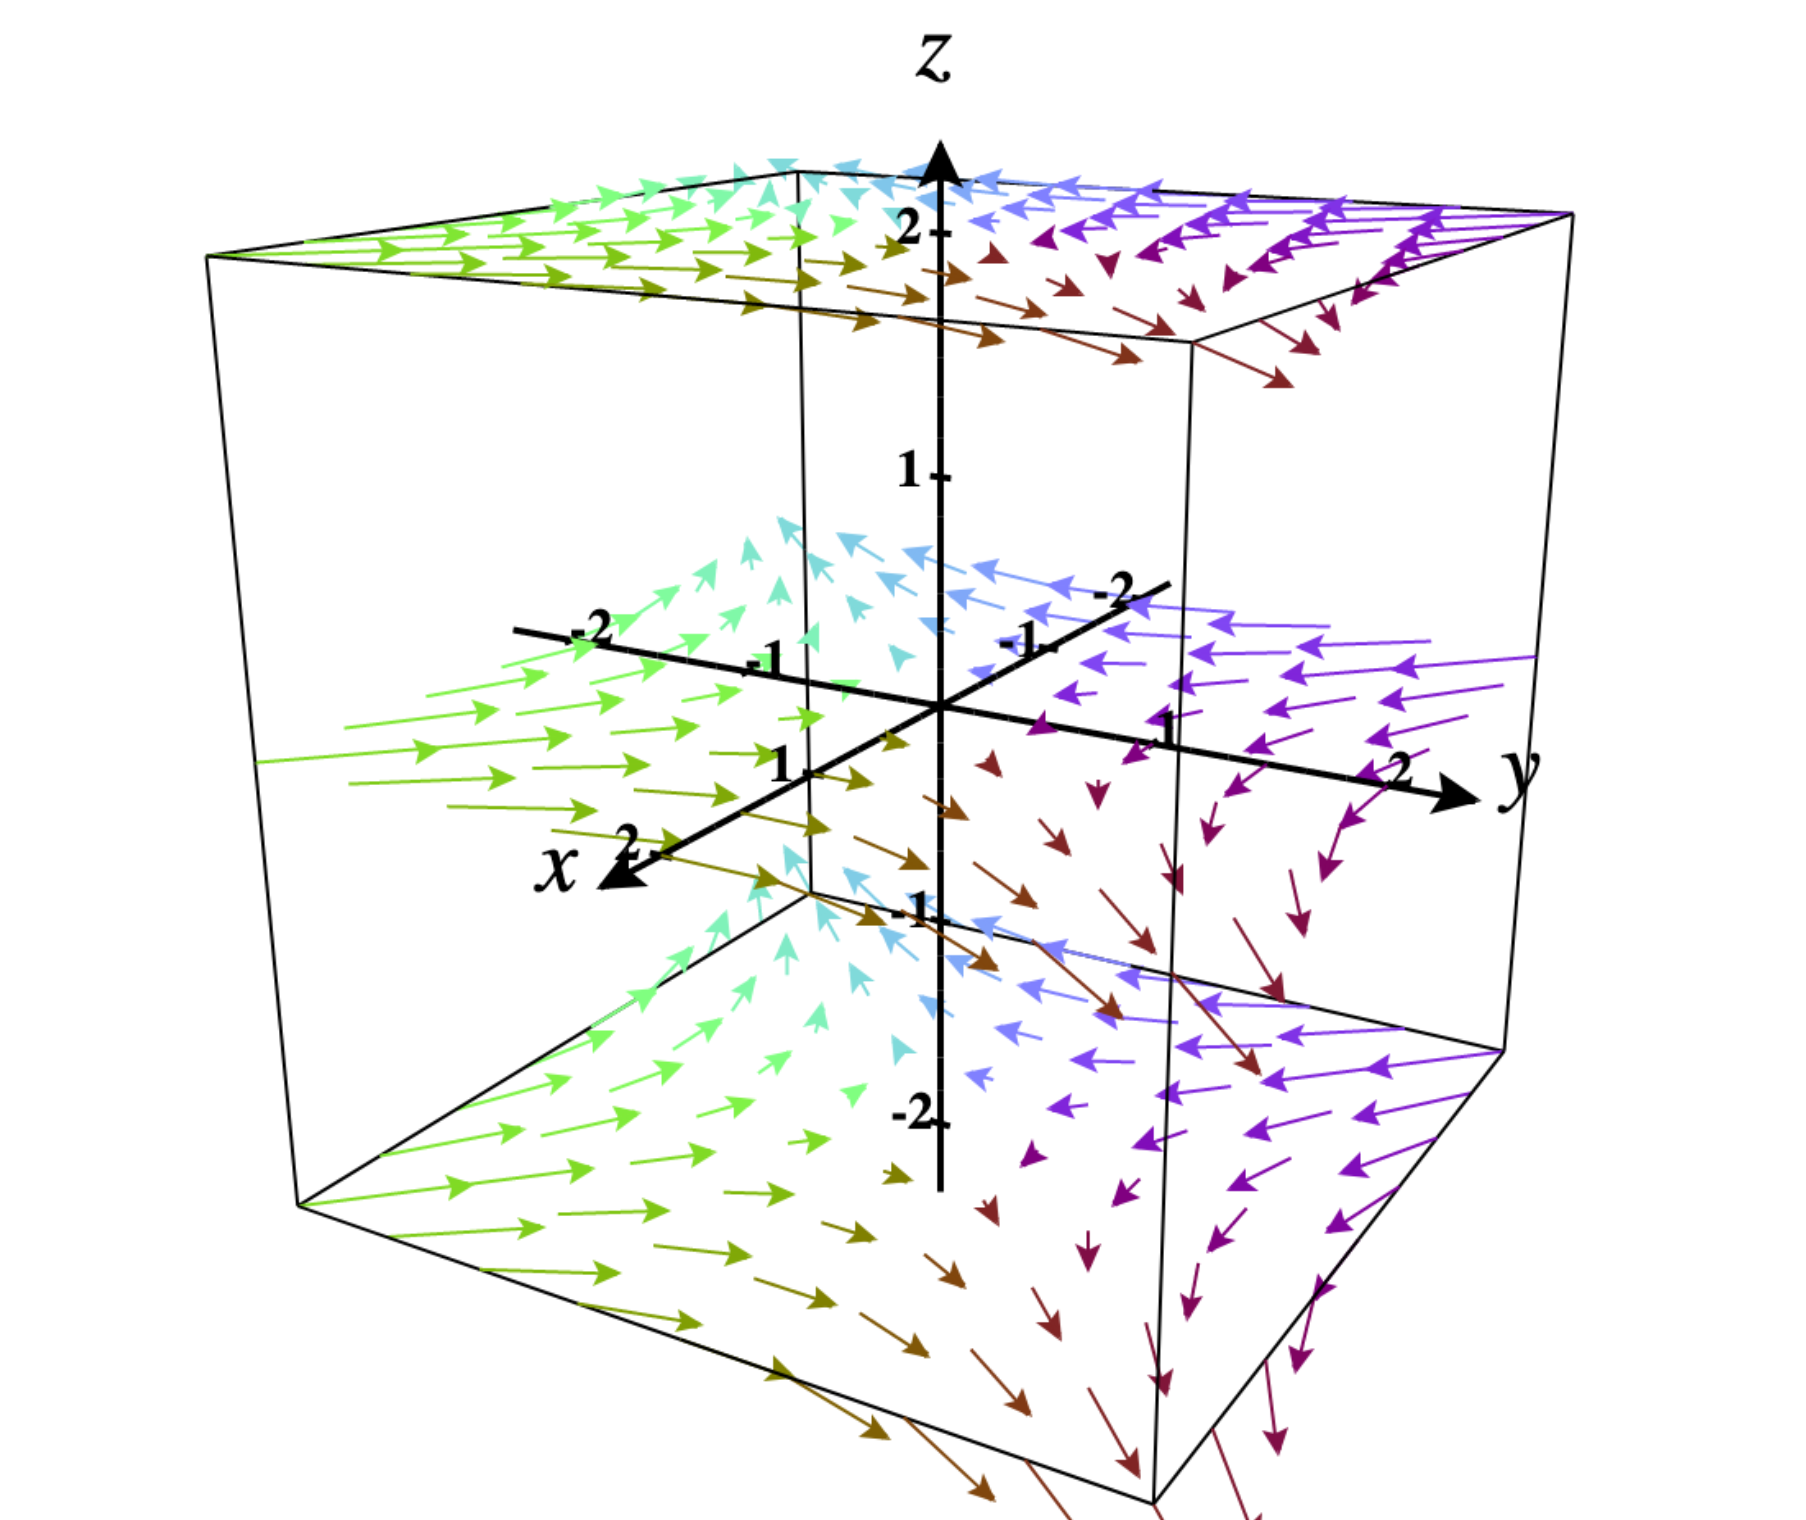
\includegraphics[width=.6\textwidth]{Images/5b.png}
        \caption{Plot for $\mathbf{w}(x,y,z)$.}
    \end{figure}
    \item 
    \begin{figure}[H]
        \centering
        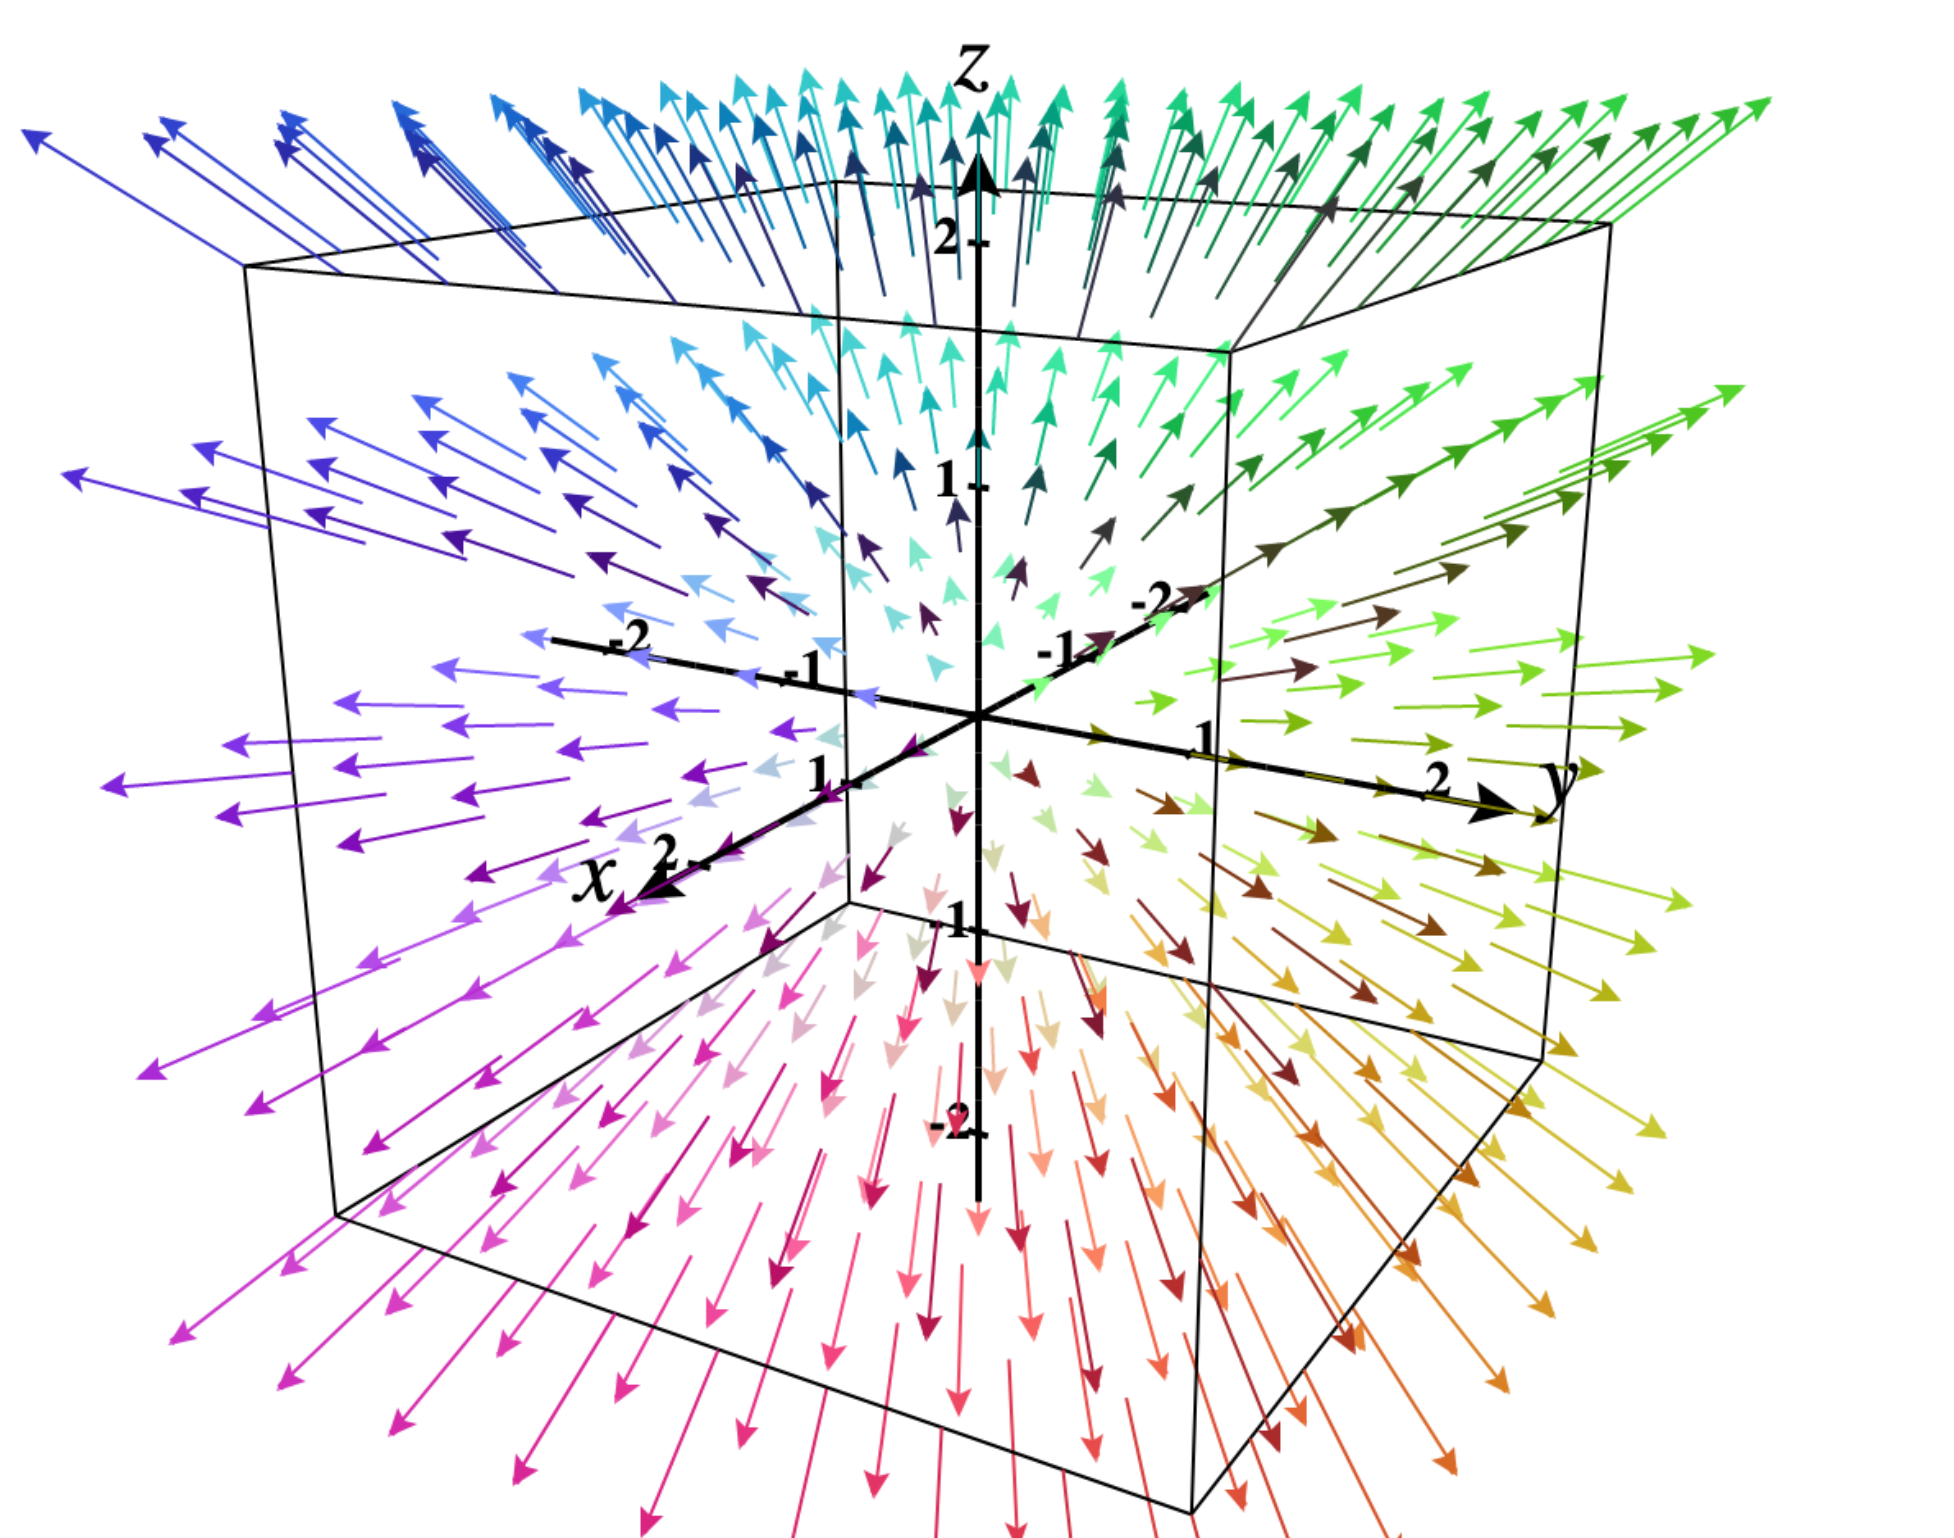
\includegraphics[width=.6\textwidth]{Images/5c.png}
        \caption{Plot for $\mathbf{u}(x,y,z)$.}
    \end{figure}
    \item 
    \begin{figure}[H]
        \centering
        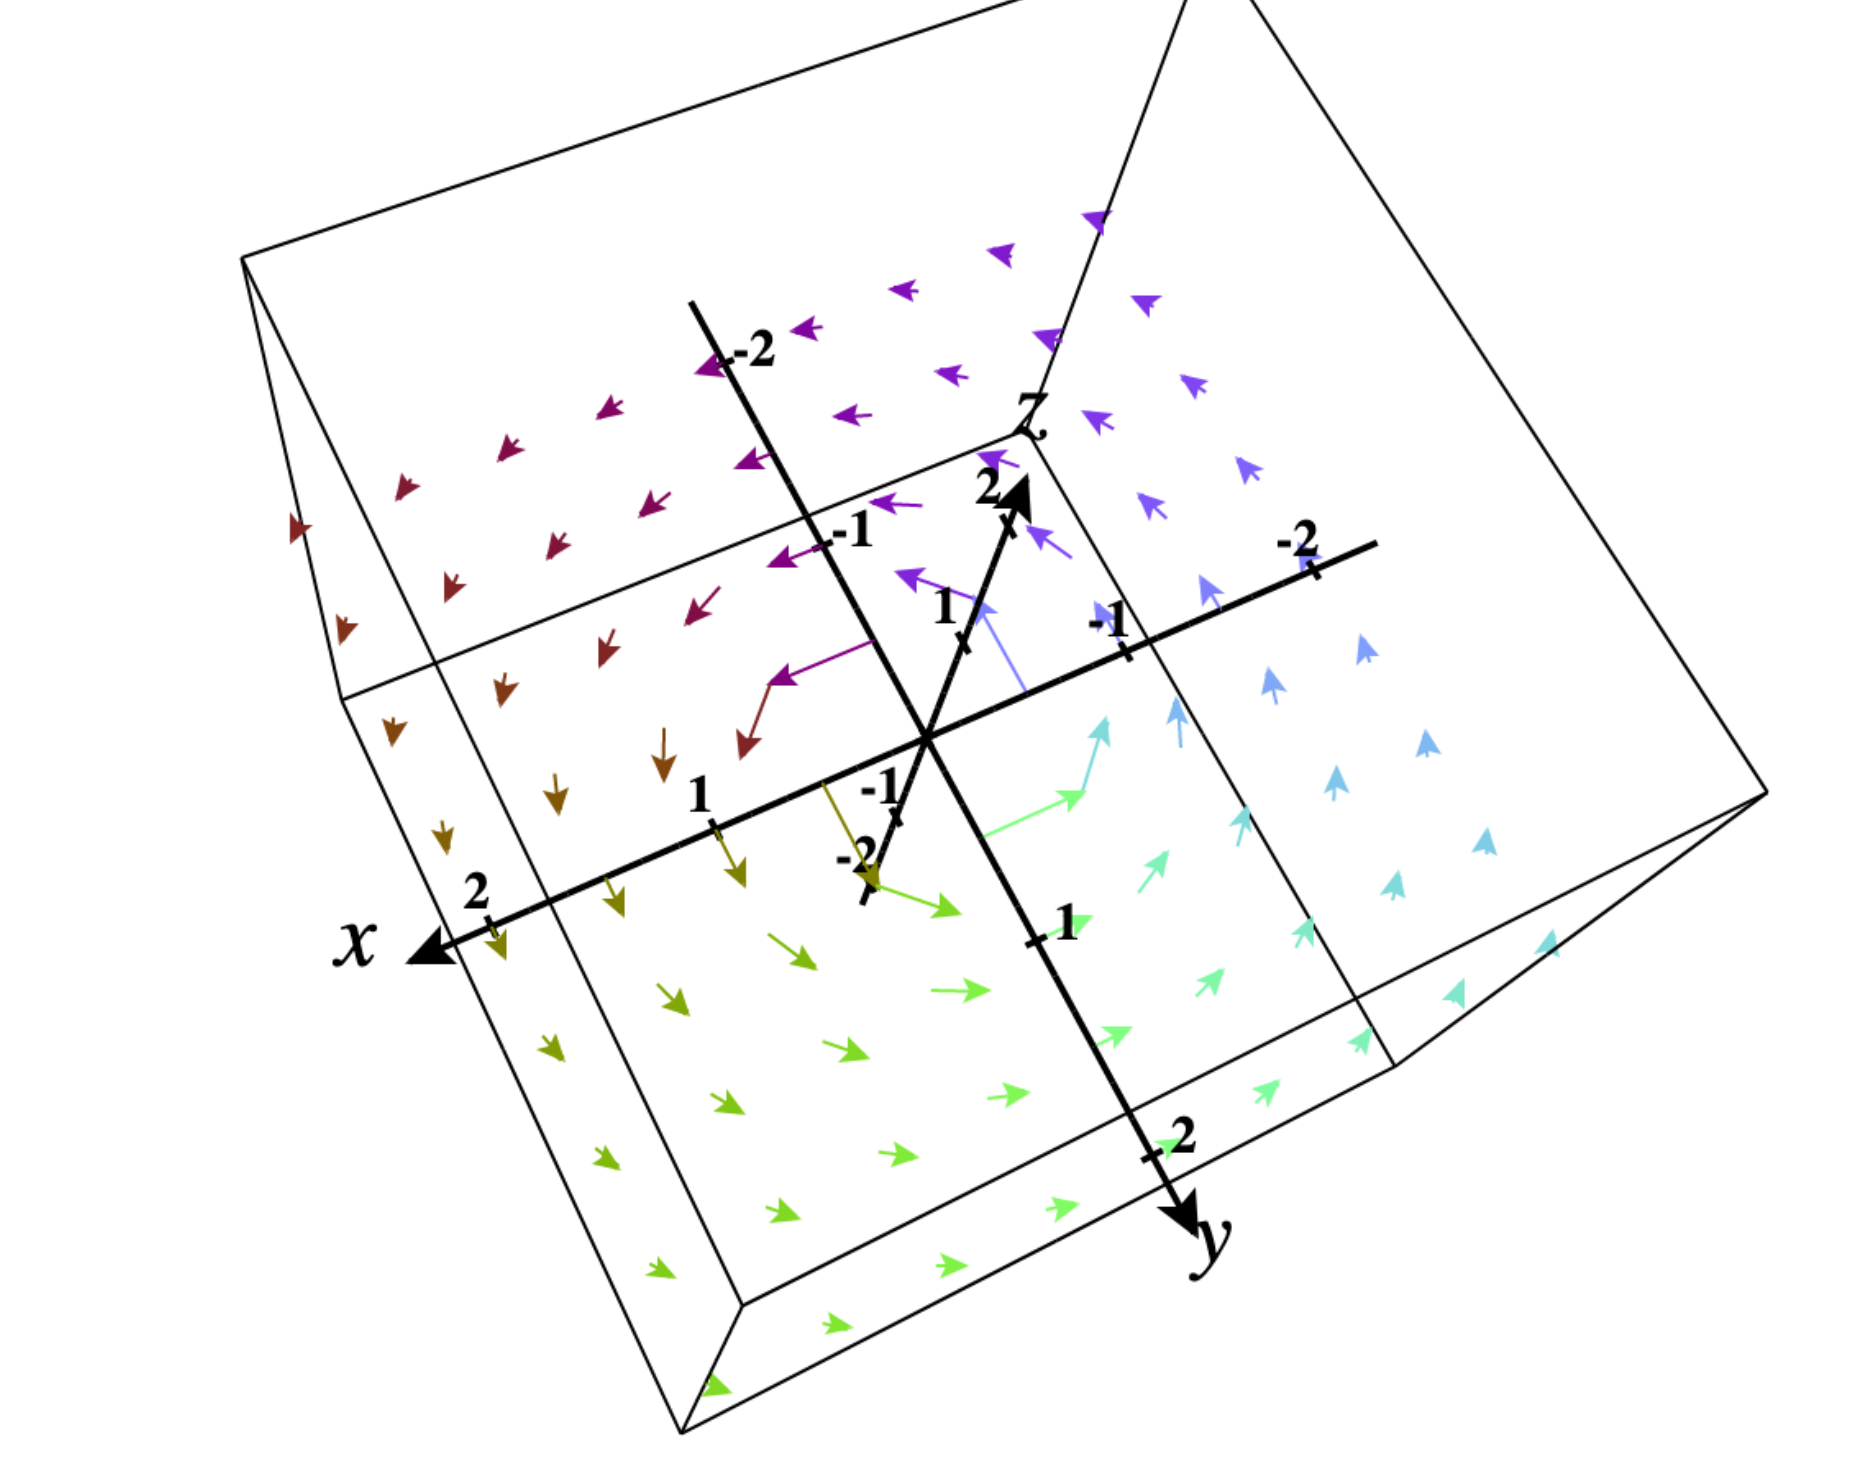
\includegraphics[width=.6\textwidth]{Images/5d.png}
        \caption{Plot for $\mathbf{r}(x,y,z)$.}
    \end{figure}
\end{enumerate}
\end{solution}



\end{document}